
\chapter{Twin Delayed Deep Deterministic Policy Gradient}

众所周知,在基于价值学习的强化学习算法中,如 DQN,函数近似误差是导致 $Q$ 值高估和次优策略的原因。
这个问题在 AC 框架中依然也存在,TD3 
提出了新的机制去最小化它对 actor (演员, 策略函数)和 critic (评论家, 估值函数)的影响。
其算法建立在双 $Q$-learning 的基础上,通过选取两个估值函数中的较小值,从而限制它对$Q$值的过高估计。

双延迟深度确定性策略梯度算法 TD3 全称中的 
Deep Deterministic policy gradient algorithm 就是 DDPG 的全称。那么 
DDPG 和 TD3 有何渊源呢?其实简单的说,TD3 就是 DDPG 的一个优化版本。
TD3相对于DDPG,主要采用了以下重要改进:
\begin{itemize}
%\setlength{\itemsep}{0pt}
%\setlength{\parsep}{0pt}
\setlength{\parskip}{0pt}
\item[1.]
Double network
\item[2.]
Critic 学习改进
\item[3.]
Actor 学习改进
\item[4.]
target policy smoothing regularization
\end{itemize}


%+++++++++++++++++++++++++++++++++++++++++++
\section{Deterministic Policy Gradient Algorithms}
%-------------------------------------------

Policy gradient algorithms are widely used in reinforcement learning problems 
with continuous action spaces. The basic idea is to represent the policy by 
a parametric probability distribution $\pi_\theta(a|s) = \mathbb{P}
[a|s; \theta]$ that stochastically selects action $a$ in state $s$ according 
to parameter vector $\theta$. Policy gradient algorithms typically proceed 
by sampling this stochastic policy and adjusting the policy parameters
in the direction of greater cumulative reward.

In this section we instead consider \emph{deterministic} policies 
$a = \mu_\theta(s)$. It is natural to wonder whether the same approach can 
be followed as for stochastic policies: adjusting the policy parameters in 
the direction of the policy gradient. It was previously believed that the 
deterministic policy gradient did not exist, or could only be obtained when
using a model. However, we show that the deterministic policy gradient does 
indeed exist, and furthermore it has a simple model-free form that simply 
follows the gradient of the action-value function. In addition, we 
show that the deterministic policy gradient is the limiting
case, as policy variance tends to zero, of the stochastic policy gradient.

%+++++++++++++++++++++++++++++++++++++++++++
\subsection{Background}

\subsubsection{Preliminaries}

We can then write the performance objective as an expectation,
\begin{eqnarray}\label{eq_DPG_performance_objective}
J(\pi_\theta) &=& \int_\mathcal{S}\rho^\pi(s)\int_\mathcal{A}\pi_\theta
(s,a) r(s,a) dads \notag \\
&=& \mathbb{E}_{s\sim\rho^\pi, a\sim\pi_\theta}[r(s,a)]
\end{eqnarray}
where $\mathbb{E}_{s\sim\rho}[\cdot]$ denotes the (improper) expected 
value with respect to discounted state distribution $\rho(s)$. In the 
remainder of this section we suppose for simplicity that $\mathcal{A} 
= \mathbb{R}^m$ and that $\mathcal{S}$ is a compact subset of $\mathbb{R}^d$.

\subsubsection{Stochastic Policy Gradient Theorem}

\emph{Policy gradient} algorithms are perhaps the most popular class of 
continuous action reinforcement learning algorithms. The basic idea behind 
these algorithms is to adjust the parameters $\theta$ of the policy in the 
direction of the performance gradient $\nabla_\theta J(\pi_\theta)$. The 
fundamental result underlying these algorithms is the \emph{policy 
gradient theorem},
\begin{eqnarray}\label{eq_DPG_policy_gradient_theorem}
\nabla_\theta J(\pi_\theta)
&=& \int_\mathcal{S}\rho^\pi(s)\int_\mathcal{A}\nabla_\theta\pi_\theta
(a|s)Q^\pi(s,a) da ds \notag \\
&=& \mathbb{E}_{s\sim\rho^\pi, a\sim\pi_\theta}
[\nabla_\theta\log\pi_\theta(a|s)Q^\pi(s,a)]
\end{eqnarray}


%+++++++++++++++++++++++++++++++++++++++++++
\subsection{Stochastic Actor-Critic Algorithms}

The {\bf actor-critic} is a widely used architecture based on the
policy gradient theorem. The actor-critic consists of two eponymous 
components. {\bf An \emph{actor} adjusts the parameters $\theta$ of the 
stochastic policy $\pi_\theta(s)$ by stochastic gradient ascent of 
Equation (\ref{eq_DPG_policy_gradient_theorem}).} Instead of the
unknown true action-value function $Q^\pi(s,a)$ in Equation 
(\ref{eq_DPG_policy_gradient_theorem}), an action-value function 
$Q^w(s, a)$ is used, with parameter vector $w$. {\bf A \emph{critic} 
estimates the action-value function $Q^w(s,a)\approx Q^\pi(s,a)$ 
using an appropriate policy evaluation algorithm such as 
temporal-difference learning.}

Actor Critic 合并了以值为基础(比如$Q$-learning)和以动作概率为基础(比如 Policy 
Gradients)的两类强化学习算法。Actor 的前身是 Policy Gradients, 
该方法可以在连续动作中选取合适的动作;Critic 的前生是 $Q$-learning 
或者其他以值为基础的学习法, 能进行单步更新, 但并不能处理连续动作。而传统的 Policy 
Gradients 则是回合更新。我们就比较贪心了,又想处理连续动作,又想单步更新,
那就你们两个结合一下呗。actor 网络输入 state,输出action;critic 网络输入为 state
和 action,输出为 $Q$ 值,就组成了 Actor Critic。但传统 Actor-Critic 
前后相关性高,学习片面,于是人们有学习了 DQN 中的方法,使用一个 Replay buffer 
和两个结构相同, 但参数更新频率不同的神经网络来训练,于是就有了 DDPG。

还有一个模型 A3C 采用多线程的方法,每个线程对应不同的探索策略,
从而达到样本间是低相关的效果,不再需要 DQN 中引入 experience replay 
机制来进行训练。这样能够采用on-policy的方法进行训练。

UNREAL 建立在 A3C 的基础上,加入多个辅助任务。A3C 算法是 on policy 
的,而辅助任务利用 A3C 中的 Replay buffer,是 off policy 的。

\begin{figure}[H]
\centering
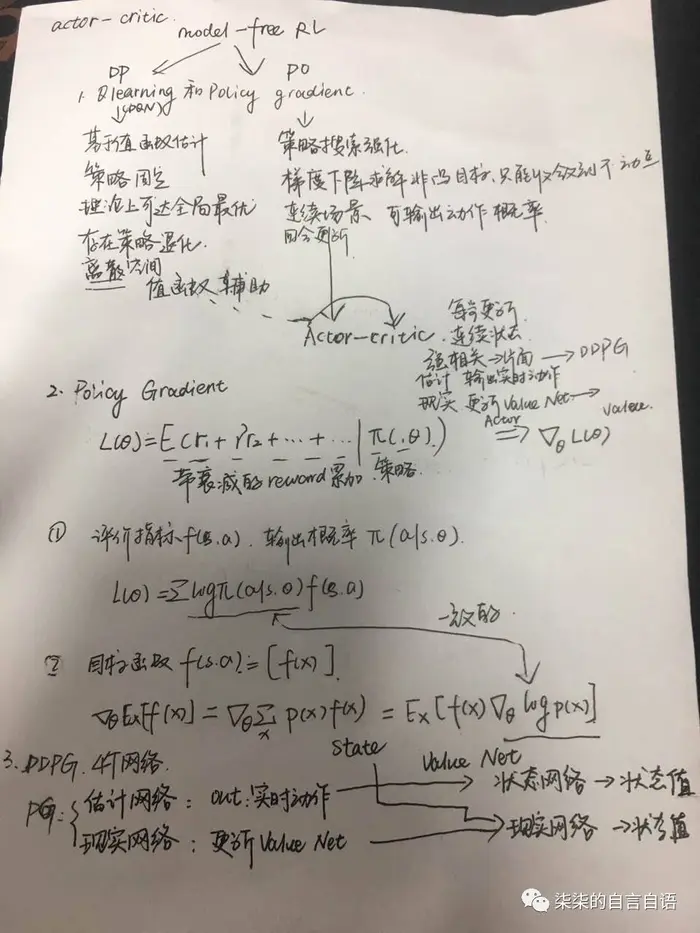
\includegraphics[scale=0.118]{pix/td3/1.png}
%\caption{Agent and Environment}
%\label{fig:label}
\end{figure}

\begin{figure}[H]
\centering
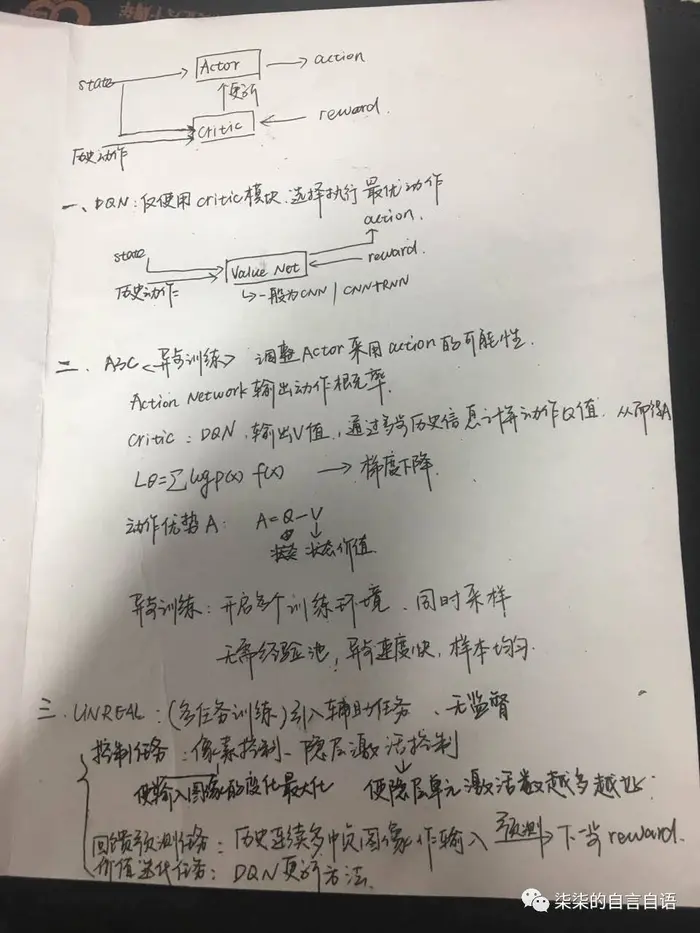
\includegraphics[scale=0.118]{pix/td3/2.png}
%\caption{Agent and Environment}
%\label{fig:label}
\end{figure}

%+++++++++++++++++++++++++++++++++++++++++++
\section{Deep Deterministic Policy Gradient (DDPG)}
%-------------------------------------------

% https://saashanair.com/blog/blog-posts/deep-deterministic-policy-gradient-ddpg-how-does-the-algorithm-work

{\bf TL; DR}: Deep Deterministic Policy Gradient, or DDPG in short, is an 
actor-critic based off-policy reinforcement learning algorithm. It combines 
the concepts of Deep $Q$ Networks (DQN) and Deterministic Policy Gradient (DPG) 
to learn a deterministic policy in an environment with a continuous action space.

The first image invoked on hearing the words "Reinforcement Learning" is often 
the DQN algorithm. Despite its success in the Atari environments, DQN only works 
within discrete action space. Most real-world applications, such as robotics, 
autonomous driving and so on, however, require the actions to have continuous-values. 
Thus, Deep Deterministic Policy Gradient (DDPG) attempts to fill this gap by 
introducing a few "tweaks" that allow DQN to be extended to continuous action space.


%+++++++++++++++++++++++++++++++++++++++++++
\subsection{The schematics}

First things first, how many neural networks do we require? DDPG is based on 
the off-policy deterministic actor-critic setting. Thus, we require at least two 
networks, one for the actor and another for the critic.

Additionally, to ensure stability during training, DDPG borrows the concept of 
target networks from DQN (参见 \ref{subsubsection_double_deep_q_network}). Thus, 
we need a total of 4 networks to run this algorithm; 
an actor $\mu$ (also represented as $\pi$ sometimes, as in the TD3 paper), a critic 
$Q$ and their respective targets, $\mu'$ and $Q'$.

\begin{figure}[H]
\centering
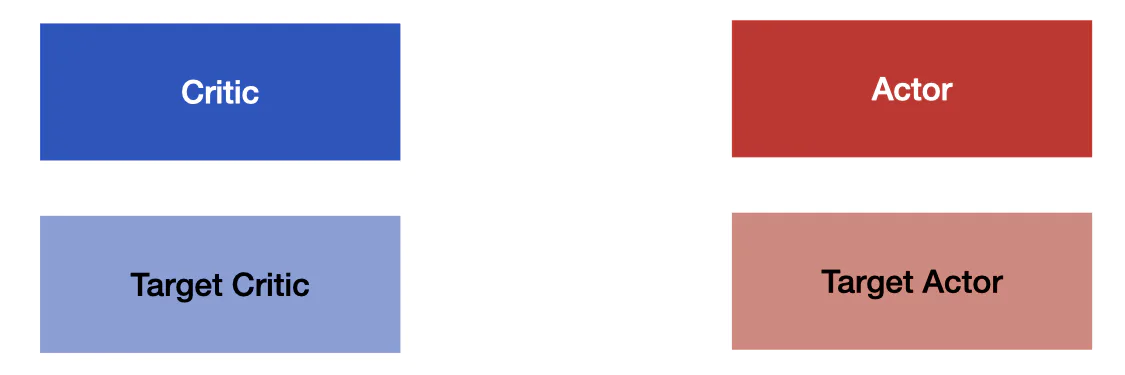
\includegraphics[scale=0.5]{pix/td3/ddpg_schematics.png}
\caption{DDPG uses a total of 4 networks - one actor, one critic and their 
corresponding targets}
%\label{fig:action_for_each_state}
\end{figure}

Being off-policy, DDPG also benefits from the use of a 'Replay Buffer', similar 
to DQN. The replay buffer is a finite-sized cache that stores past experiences 
from which batches are sampled uniformly at random for training.

%+++++++++++++++++++++++++++++++++++++++++++
\subsection{The DDPG Critic}

As the name suggests, the task of the critic is to "critique" the actor's beliefs 
by determining 'how good is the suggested action given the current state'. In other 
words, the critic is tasked with computing the $Q$-value $Q(s,a)$ of the given 
state-action pair.

"Wait! So if we are in any case computing the $Q$-value, why not directly use DQN 
then?", you might wonder. Let's for a minute think back to how the $Q$-value was 
computed in DQN. In the DQN setting, the state is given as input to the network, 
while at the other end we generate '$n$' $Q$-values, one for each of the possible 
discrete actions. To select the action to be performed, we pick the action with 
the highest $Q$-value. Computing $Q$-values for all possible actions makes sense 
when we have a small number of discrete actions to pick from. But in situations 
where we need to train an RL agent to control a robotic arm or drive an autonomous 
vehicle, it isn't sufficient to just say 'turn left', we need to specify 'by how 
much' we need it to turn. We, thus, need a continuous action space to allow for 
such fine-grained control.

"So, how does DDPG compute the $Q$-value then?", you may ask. Since DDPG delegates 
the responsibility of predicting the action and determining the "goodness" of that 
action to two different networks, the critic must only compute the $Q$-value based 
on the action selected by the other network. Thus, the input to the critic, here, 
is the state and the predicted action, while the output layer of the network has a 
single neuron that produces the $Q$-value of the given state-action pair.

\begin{figure}[H]
\centering
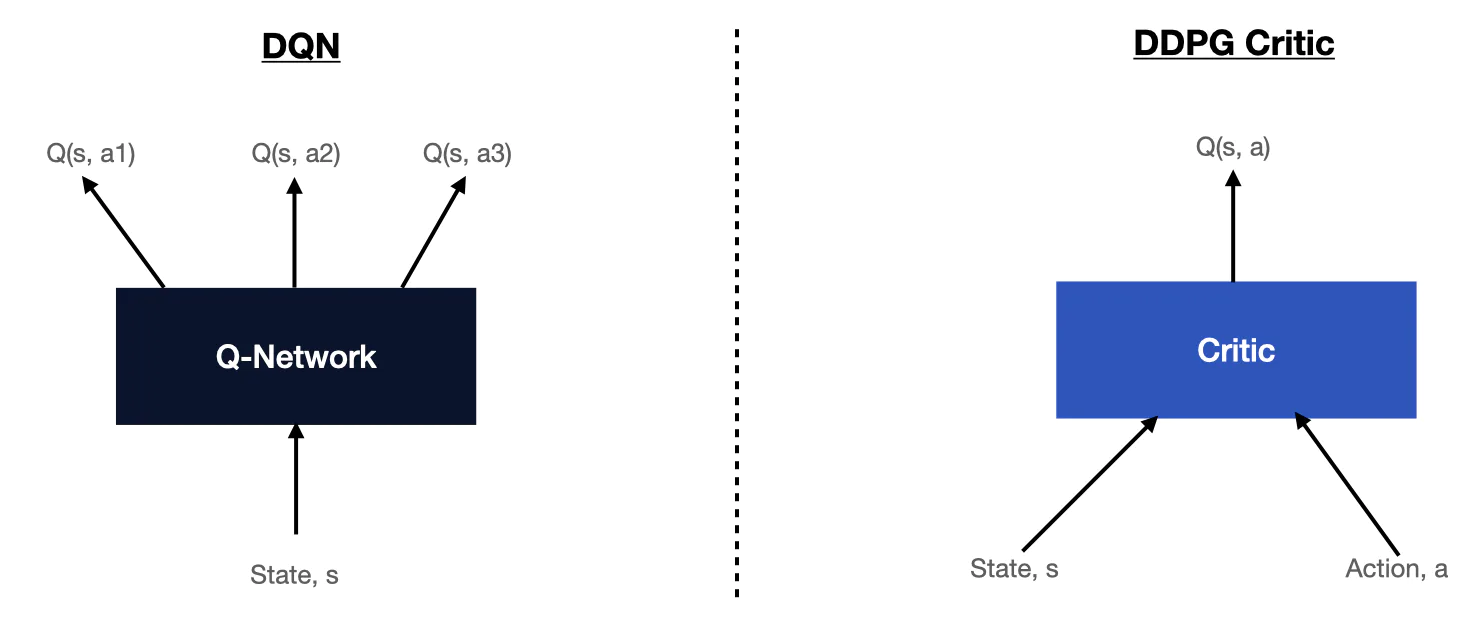
\includegraphics[scale=0.5]{pix/td3/ddpg_critic.png}
\caption{Calculation of Q-values in DQN vs DDPG Critic}
%\label{fig:action_for_each_state}
\end{figure}

The next natural question is, "How does the critic network learn?" The Mean-Squared 
Bellman Error is used, similar to DQN. Thus, the loss is computed as the Mean-Squared 
Error between the TD-Target and the $Q$-value estimate of the current state and 
corresponding action. The TD-Target $y$ utilises the target networks. The next state 
$s'$ and the associated action predicted by the target actor $\mu'$ are provided as 
input to the target critic $Q'$. This can be formulated as:
$$
y = r + \gamma \cdot Q'(s', \mu'(s'))
$$

\begin{figure}[H]
\centering
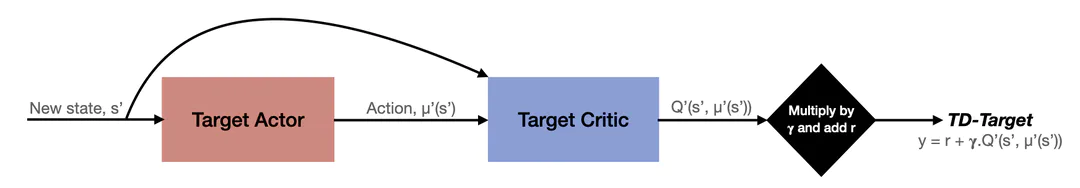
\includegraphics[scale=0.5]{pix/td3/ddpg_critic_loss.png}
\caption{Calculation of TD-Target that is used in the Critic Loss}
%\label{fig:action_for_each_state}
\end{figure}


%+++++++++++++++++++++++++++++++++++++++++++
\subsection{The DDPG Actor}

Being based on DPG, the DDPG agent learns a deterministic policy. This means that 
the actor-network learns to map a given state to a specific action, instead of a 
probability distribution on the actions, as is done in algorithms that learn a 
stochastic policy. Thus, the actor-network takes as input the state vector and 
outputs the action to be performed, with the size of the layer dependent on the 
size of the action space.

The actor-network improves based on the "critique" of the critic network. Thus, 
based on the Deterministic Policy Gradient Theorem (which we will get into at a 
later date), the actor-network learns by performing a gradient ascent (thereby 
requiring the negative sign indicated below for implementation with autodiff), 
with respect to the policy, along the direction indicated by the critic. This 
can be formulated as:
$$
L_{\text{actor}} = - Q(s, \mu(s))
$$

\begin{figure}[H]
\centering
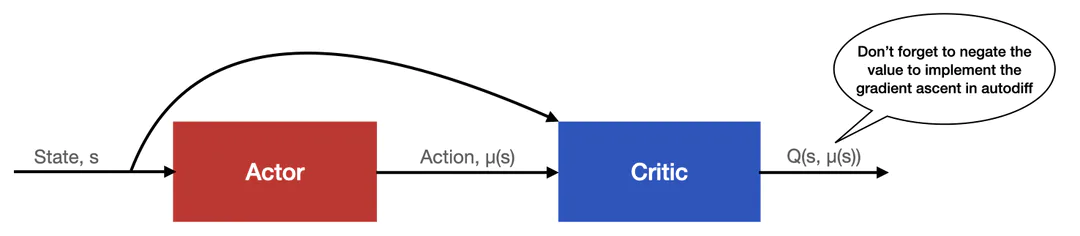
\includegraphics[scale=0.5]{pix/td3/ddpg_actor_loss.png}
\caption{Calculation of the Actor Loss}
%\label{fig:action_for_each_state}
\end{figure}


%+++++++++++++++++++++++++++++++++++++++++++
\subsection{Updating the DDPG Targets}

Target networks were introduced in DDPG to deal with the instability caused due to the use of the 
Bellman Error. Since the critic updates in DDPG depend on the Bellman Error, target networks 
become necessary. However, the two algorithms differ in the way that the targets are updated.

DQN works by applying hard updates, i.e., periodically the weights of the main network are copied 
into the target network directly. In contrast, DDPG performs 'soft updates' at each training step. 
As indicated below, Polyak averaging is used for this:

\begin{eqnarray*}
\theta' &\leftarrow& \tau \cdot \theta + (1 - \tau) \cdot \theta' \\
\phi' &\leftarrow& \tau \cdot \phi + (1 - \tau) \cdot \phi' \notag
\end{eqnarray}
Here, $\theta$ and $\theta'$ represent the parameters of the critic and the target critic networks 
respectively, while $\phi$ and $\phi'$ represent the parameters of the actor and its target. The 
hyperparameter $\tau \in [0, 1]$ is set to an extremely small value to ensure that the targets update 
very slowly.

% https://saashanair.com/blog/blog-posts/deep-deterministic-policy-gradient-ddpg-how-does-the-algorithm-work





%+++++++++++++++++++++++++++++++++++++++++++
\section{TD3 对 DDPG 的改进}
%-------------------------------------------

在强化学习中,对于离散化的动作的学习,都是以 DQN 为基础的。DQN 通过的
$\arg\max\Q_{\text table}$的方式去选择动作。这往往会过大估计价值函数,从而造成误差。

在连续的动作控制的 AC 框架中,如果每一步都采用这种方式去估计,将导致误差累积,
从而导致无法找到最优策略,最终致使算法无法收敛。

因此,TD3 对 DDPG 做了如下改进:
\begin{itemize}
\item[-]
使用两个 Critic 网络。使用两个网络对动作价值函数进行估计,(这与 Double DQN 
的思想差不多)。在训练的时候选择 $\min\left( Q^{\theta_1}(s,a), Q^{\theta_2}(s,a) \right)$ 
作为估计值。

\item[-]
使用软更新的方式 。不再采用直接复制,而是使用 $\theta = \tau\theta' + (1 - \tau) 
\theta$ 更新网络参数。

\item[-]
使用策略噪音。使用 Epsilon-Greedy 在探索的时候使用了探索噪音。
(用策略噪声在更新参数的时候来平滑策略期望)

\item[-]
使用延迟学习。Critic 网络更新的频率要比 Actor 网络更新的频率要大。

\item[-]
使用梯度截取。将Actor的参数更新的梯度截取到某个范围内。
\end{itemize}

DDPG 中的网络架构如下面图\ref{fig:ddpg_net_architecture}。
\begin{figure}[H]
\centering
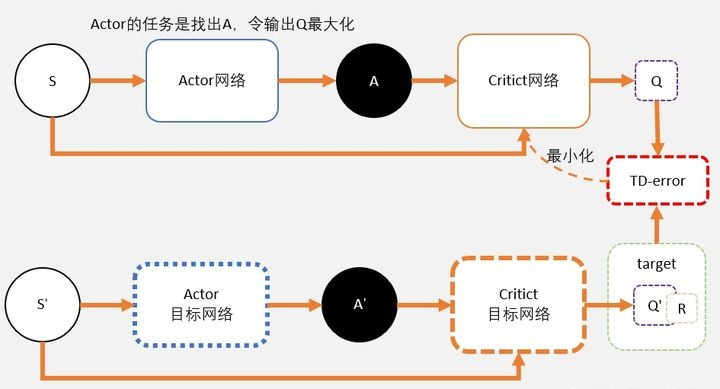
\includegraphics[scale=0.618]{pix/td3/ddpg_architecture.jpg}
\caption{DDPG 网络架构}
\label{fig:ddpg_net_architecture}
\end{figure}

TD3 通过 Critic 网络估算动作的 A 值。一个 Critic 的评估可能会较高,所以我们加一个。
如是 TD3 的网络架构如图\ref{fig:td3_net_architecture}所示。
\begin{figure}[H]
\centering
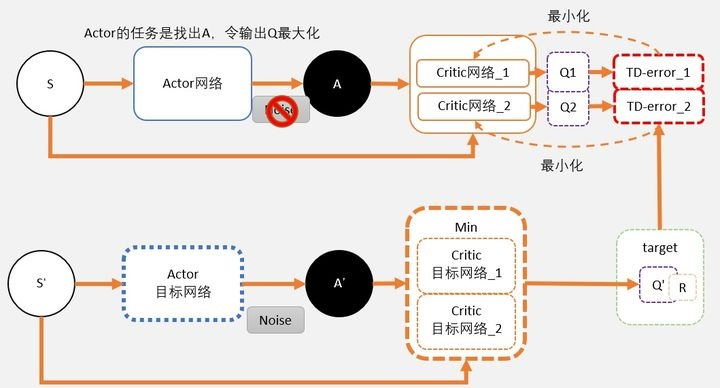
\includegraphics[scale=0.618]{pix/td3/td3_architecture.jpg}
\caption{TD3 网络架构}
\label{fig:td3_net_architecture}
\end{figure}

在目标网络中,我们估算出来的 $Q$ 值会用min()函数求出较少值。以这个值作为更新的目标。
这个目标会更新两个网络 Critic网络1 和 Critic网络2。
你可以理解为这两个网络是完全独立,他们只是都用同一个目标进行更新。
剩余的就和 DDPG 一样了。过一段时间,把学习好的网络赋值给目标网络。


%+++++++++++++++++++++++++++++++++++++++++++
\subsection{Objective}

Similar to Deep $Q$-Networks, the problem of overestimation of the state values, occuring 
due to noisy function approximators and using the same function approximator for action 
selection and value estimation also persists in actor-critic algorithms with continuous 
action-spaces. Double DQN, the solution for this problem in Deep $Q$-Networks is not 
effective in actor-critic algorithms due to the slow rate of change of the policy. Twin 
Delayed DDPG (TD3) uses Clipped Double $Q$-Learning to address this problem. TD3 uses two 
$Q$ function approximators and the loss function for each is given by
\begin{align*}
L(\phi_{1}, \mathcal{D}) = E_{(s,a,r,s',d) \sim \mathcal{D}}[(Q_{\phi_{1}}(s, a) - y(r,s',d))^2] \\
L(\phi_{2}, \mathcal{D}) = E_{(s,a,r,s',d) \sim \mathcal{D}}[(Q_{\phi_{2}}(s, a) - y(r,s',d))^2]
\end{align}


%+++++++++++++++++++++++++++++++++++++++++++
\subsection{Clipped Double $Q$-Learning}

Double DQNs are not effective in actor-critic algorithms due to the slow change in the policy 
and the original double $Q$-Learning (although being somewhat effective) does not completely 
solve the problem of overestimation. To tackle this TD3 uses Clipped Double $Q$-Learning 
Clipped. Double $Q$-Learning proposes to upper bound the less biased critic network by the 
more biased one and hence no additional overestimation can be introduced. Although, this may 
introduce underestimation, it is not much of a concern since underestimation errors don't 
propagate through policy updates. The target function calculated usign Clipped Double 
$Q$-Learning for the updates can be written as
$$
y = r + \gamma \min_{i=1,2}Q_{\theta_i'}(s', \pi_{\phi_1}(s'))
$$
Both of the critic networks are updated using the loss functions mentioned above.


%+++++++++++++++++++++++++++++++++++++++++++
\subsection{Experience Replay}

TD3 being an off-policy algorithm, makes use of Replay Buffer. Whenever a transition 
$(s_t, a_t, r_t, s_{t+1})$ is encountered, it is stored into the replay buffer. Batches of 
these transitions are sampled while updating the network parameters. This helps in breaking 
the strong correlation between the updates that would have been present had the transitions 
been trained and discarded immediately after they are encountered and also helps to avoid 
the rapid forgetting of the possibly rare transitions that would be useful later on.

\begin{lstlisting}[language=Python]
def log(self, timestep: int) -> None:
    """Helper function to log

    Sends useful parameters to the logger.

    Args:
        timestep (int): Current timestep of training
    """
    self.logger.write(
        {
            "timestep": timestep,
            "Episode": self.episodes,
            **self.agent.get_logging_params(),
            "Episode Reward": safe_mean(self.training_rewards),
\end{lstlisting}


%+++++++++++++++++++++++++++++++++++++++++++
\subsection{The TD3 Critic}

只有我们在计算 Critic 的更新目标时,我们才用 target network。其中就包括了一个 Policy 
network,用于计算 $A'$;两个 $Q$ network ,用于计算两个 $Q$ 值:$Q_1(A')$ 和 $Q_2(A')$。

$Q_1(A')$ 和 $Q_2(A')$ 取最小值 $\min(Q_1,Q_2)$ 将代替 DDPG 的 $Q(a')$ 
计算更新目标,也就是说: $\text{target} = \min(Q_1,Q_2) * \gamma + r$。
target 将会是 $Q\_network\_1$ 和 $Q\_network\_2$ 两个网络的更新目标。

既然更新目标是一样的,那么为什么还需要两个网络呢?

虽然更新目标一样,两个网络会越来越趋近与和实际 $q$ 值相同。但由于网络参数的初始值不一样,
会导致计算出来的值有所不同。所以我们可以有空间选择较小的值去估算 $q$ 值,避免 $q$ 值被高估。


%+++++++++++++++++++++++++++++++++++++++++++
\subsection{The TD3 Actor}

可以将网络的图像想象成一张布,覆盖在 $q$-table 上。当我们输入某个状态的时候,相当于这块布上的一个截面,
我们我们能够看到在这个状态下的一条曲线。

而 actor 的任务,就是用梯度上升的方法,寻着这条线的最高点。

对于 actor 来说,其实并不在乎 $Q$ 值是否会被高估,其任务只是不断做梯度上升,寻找这条最大的 $Q$ 
值。随着更新的进行 $Q_1$ 和 $Q_2$ 两个网络,将会变得越来越像。所以用 $Q_1$ 还是 $Q_2$,
还是两者都用,对于 actor 的问题不大。


%+++++++++++++++++++++++++++++++++++++++++++
\subsection{Delayed Policy updates}

这里的 Dalayed,是 actor 更新的 delay。也就是说相对于 critic 可以更新多次后,actor 再进行更新。

$Q$-network 在学习过程中,我们的 $q$ 值是不断变化的,也就是说 $Q$-table 所在的布是不断变形的。
所以要寻着最高点的任务有时候就难为 actor 的了。可以想象,本来是最高点的,当 actor 好不容易去到最高点时,
$q$ 值更新了,这个刚到达的点现在并不是最高点了。这时候 actor 只能转头再继续寻找新的最高点。
更坏的情况可能是 actor 被困在次高点,没有找到正确的最高点。

所以我们可以把 Critic 的更新频率,调的比 Actor 要高一点。让 critic 更加确定,actor 再行动。

也就是说 TD3 更新策略网络(及其 Target 网络)的频率要比价值网络慢,论文中推荐更新两次价值网络才更新一次策略网络。
这样可以让两者解耦,关联度降低,从而可以克服 over estimation。

TD3 uses target networks similar to DDPG and DQNs for the two critics and the actors to 
stabilise learning. Apart from this, it also promotes updating the policy networks at a 
lower frequency as compared to the $Q$-networks to avoid divergent behaviour for the policy. 
The paper recommends one policy update for every two Q-function updates.

\begin{lstlisting}[language=Python]
def update_params(self, update_interval: int) -> None:
    """Update parameters of the model

    Args:
        update_interval (int): Interval between successive updates of the 
        target model
    """
    for timestep in range(update_interval):
        batch = self.sample_from_buffer()

        value_loss = self.get_q_loss(batch)

        self.optimizer_value.zero_grad()
        value_loss.backward()
        self.optimizer_value.step()

        # Delayed Update
        if timestep % self.policy_frequency == 0:
            policy_loss = self.get_p_loss(batch.states)

            self.optimizer_policy.zero_grad()
            policy_loss.backward()
            self.optimizer_policy.step()

            self.logs["policy_loss"].append(policy_loss.item())
            self.logs["value_loss"].append(value_loss.item())
\end{lstlisting}


%+++++++++++++++++++++++++++++++++++++++++++
\subsection{Target Policy Smoothing Regularization}

TD3 adds noise to the target action to reduce the variance induced by function 
approximation error. This acts as a form of regularization which smoothens the 
changes in the action-values along changes in action

\begin{align*}
a &= \pi_{\phi'}(s') + \epsilon \\
\epsilon &\sim \text{clip}(\mathcal{N}(0, \sigma), -c, c)
\end{align}

TD3 在策略网络的 target 网络中引入了噪声,让其更加积极去探索 $Q$ 价值网络的错误。
\begin{align*}
a_\text{TD3}(s') &= \text{clip}(\mu_{\theta,targ}(s') + \text{clip}(\epsilon,−c,c), 
a_\text{low},a_\text{high}), \\
\epsilon &\sim \mathcal{N}(0,\sigma)
\end{align}

价值函数的更新目标每次都在 action 上加一个小扰动,这个操作就是 target policy smoothing regularization

为什么要这样呢?

回到关于 $Q$-table “布”的类比(离散时有 $Q$-table,连续情况呈现连续的分布象一张 $Q$-table 布)。
在 DDPG 中,计算 target 的时候,我们输入时 $s'$ 和 $a'$,获得 $q$,也就是这块布上的一点 $A$。
通过估算 target 估算另外一点 $(s,a)$,也就是布上的另外一点 $B$ 的 $Q$ 值。

\begin{figure}[H]
\centering
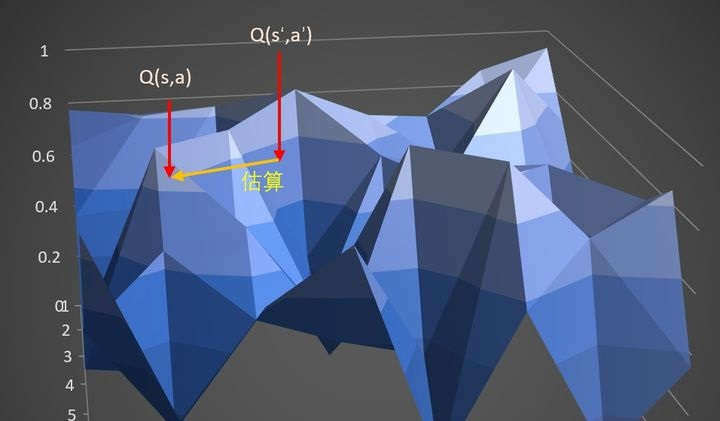
\includegraphics[scale=0.618]{pix/td3/q_table_distribution.jpg}
\caption{$Q$-distribution}
%\label{fig:label}
\end{figure}

在 TD3 中,计算 target 时候,输入 $s'$ 到 actor 输出 $a'$ 后,给 $a'$ 加上噪音,让 $a'$ 
在一定范围内随机。这又什么好处呢。好处就是,当更新多次的时候,就相当于用 $A$ 点附近的一小部分范围
(准确来说是在 $s'$ 这条线上的一定范围)的去估算 $B$,这样可以让 $B$ 点的估计更准确,更健壮。

\begin{figure}[H]
\centering
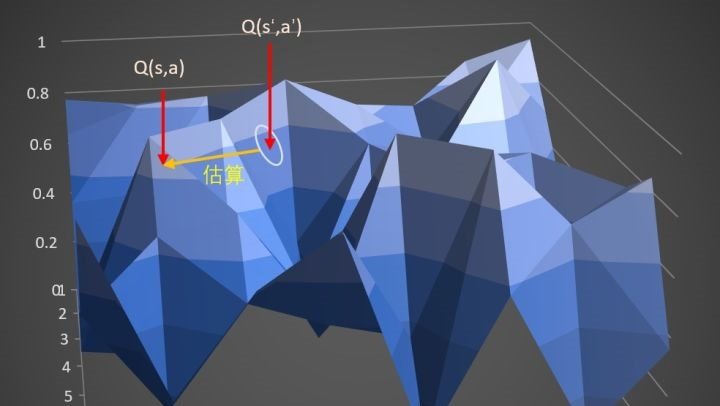
\includegraphics[scale=0.618]{pix/td3/perturbed_in_q_distribution.jpg}
\caption{perturbed $Q$-distribution}
%\label{fig:label}
\end{figure}

注意三点区分:
\begin{itemize}
%\setlength{\itemsep}{0pt}
%\setlength{\parsep}{0pt}
\setlength{\parskip}{0pt}
\item[(1)]
在跑游戏的时候,我们同样加上了 noise。这个时候的 noise 是为了更充分地开发整个游戏空间。
\item[(2)]
计算 target 的时候,actor 加上 noise,是为了预估更准确,网络更有健壮性。
\item[(3)]
更新 actor 的时候,我们不需要加上 noise,这里是希望 actor 能够寻着最大值。加上 noise 并没有任何意义。
\end{itemize}


%+++++++++++++++++++++++++++++++++++++++++++
\subsection{TD3 算法流程}

Initialize critic networks $Q_{\theta_1}, Q_{\theta_2}$, and actor 
network $\pi_\phi$ with random parameters $\theta_1$, $\theta_2$, $\phi$ 

Initialize target networks $\theta'_1 \leftarrow \theta_1$, 
$\theta'_2 \leftarrow \theta_2$, $\phi' \leftarrow \phi$ 

Initialize replay buffer $\mathcal{B}$ 

{\bf for} $t=1$ {\bf to} $T$ {\bf do} 

	\setlength\parindent{4em}
	Select action with exploration noise $a\sim\pi_\phi(s) + \epsilon$,
		$\epsilon\sim\mathcal{N}(0, \sigma)$ and observe reward $r$ and new state $s'$

	\setlength\parindent{4em}
	Store transition tuple $(s,a,r,s')$ in $\mathcal{B}$

	\setlength\parindent{4em}
	Sample mini-batch of $N$ transitions $(s,a,r,s')$ from $\mathcal{B}$: 
		$\tilde{a} \leftarrow \pi_{\phi'}(s') + \epsilon$,
		$\epsilon\sim\text{clip}(\mathcal{N}(0,\theta), -c, c)$ 

		\setlength\parindent{5em}
		$y \leftarrow r + \gamma\min_{i=1,2}Q_{\theta'_i} (s',\tilde{a})$

	\setlength\parindent{4em}
	Update critics $\theta_i \leftarrow \arg\min_{\theta_i} 
	N^{-1}\sum\left(y-Q_{\theta_i}(s,a)\right)^2$

	\setlength\parindent{4em}
	{\bf if} $t$ mod $d$ {\bf then}
		
		\setlength\parindent{6em}
		Update $\phi$ by the deterministic policy gradient: 

		\setlength\parindent{7em}
		$
		\nabla_\phi J(\phi) = N^{-1}\sum\nabla_a Q_{\theta_i}(s,a)|_{a=\pi_\phi(s)}
		\nabla_\phi\pi_\phi(s)
		$

		\setlength\parindent{6em}
		Update target networks: 

		\setlength\parindent{7em}
		$
		\theta'_i\leftarrow\tau\theta_i + (1-\tau)\theta'_i
		$,
		$
		\phi'\leftarrow\tau\phi + (1-\tau)\phi'
		$

	\setlength\parindent{4em}
	{\bf end if}

\setlength\parindent{2em}
{\bf end for}

上面的流程大致是:

首先初始化3个网络,分别为$Q_{\theta_1}, Q_{\theta_2}, \pi_\phi$,随机参数
$\theta_1, \theta_2, \phi$;

接着再初始化3个Target网络,将前面初始化好的3个网络参数分别复制给对应的target网络:

\setlength\parindent{3em}
$\theta'_1 \leftarrow \theta_1$, 
$\theta'_2 \leftarrow \theta_2$, 
$\phi' \leftarrow \phi$ 。

\setlength\parindent{2em}
初始化Replay Buffer $\mathcal{B}$。

然后通过循环迭代,一次次找到最优策略。每次迭代,在选择action的值的时候加入了噪音,
使$a\sim\pi_\phi(s) + \epsilon$,$\epsilon\sim\mathcal{N}(0, \sigma)$。

然后将$(s,a,r,s')$放入$\mathcal{B}$。

然后从$\mathcal{B}$中随机采样出Mini-Batch个数据,通过
$\tilde{a} \leftarrow \pi_{\phi'}(s') + \epsilon$,
$\epsilon\sim\text{clip}(\mathcal{N}(0,\theta), -c, c)$,
计算出$s'$状态下对应的Action的值$\tilde{a}$。

通过$s'$,$\tilde{a}$,计算出target$Q_1$,target$Q_1$,
进而获取$\min\{\text{target}Q_1, \text{target}Q_2\}$并将其作为$s'$的target$Q$值。

通过贝尔曼方程计算$s$的target$Q$值,通过两个Current网络根据$s,a$分别计算出当前的
$Q$值,再将两个当前网络的$Q$值和target$Q$值通过MSE计算Loss,更新参数。

Critic网络更新之后,Actor网络则采用了延时更新,(一般采用Critic更新2次,Actor更新1次)。
通过梯度上升的方式更新Actor网络。通过软更新的方式,更新target网络。

\begin{itemize}
\item[-]
为什么在更新Critic网络时,在计算Action值的时候加入噪音,是为了平滑前面加入的噪音。

\item[-]
贝尔曼方程:针对一个连续的MRP(Markov Reward Process)的过程(连续的状态奖励过程),
状态$s$转移到下一个状态$s'$的概率的固定的,与前面的几轮状态无关。其中,
$V$表示一个对当前状态state 进行估值的函数。$\gamma$一般为趋近于$1$,但是小于$1$。
$$
V_*(s) = \max_a R^a_s + \gamma \sum_{s'\in \mathcal{S}}P^a_{ss'}V_*(s')
$$

\end{itemize}



%+++++++++++++++++++++++++++++++++++++++++++
\subsection{代码实现}


\subsubsection{搭建网络结构}

\begin{lstlisting}[language=Python]
class Actor(nn.Module):
    def __init__(self, state_dim, action_dim, max_action):
        super(Actor, self).__init__()
        self.f1 = nn.Linear(state_dim, 256)
        self.f2 = nn.Linear(256, 128)
        self.f3 = nn.Linear(128, action_dim)
        self.max_action = max_action
    def forward(self,x):
        x = self.f1(x)
        x = F.relu(x)
        x = self.f2(x)
        x = F.relu(x)
        x = self.f3(x)
        return torch.tanh(x) * self.max_action
\end{lstlisting}

下面是 critic 网络的定义,可以看到它含有 $Q_1$ 及 $Q_2$ 两个网络
\begin{lstlisting}[language=Python]
class Critic(nn.Module):
    def __init__(self, state_dim, action_dim):
        super(Critic,self).__init__()

		# Q1 architecture
        self.f11 = nn.Linear(state_dim+action_dim, 256)
        self.f12 = nn.Linear(256, 128)
        self.f13 = nn.Linear(128, 1)

		# Q2 architecture
        self.f21 = nn.Linear(state_dim + action_dim, 256)
        self.f22 = nn.Linear(256, 128)
        self.f23 = nn.Linear(128, 1)

    def forward(self, state, action):
        sa = torch.cat([state, action], 1)

        x = self.f11(sa)
        x = F.relu(x)
        x = self.f12(x)
        x = F.relu(x)
        Q1 = self.f13(x)

        x = self.f21(sa)
        x = F.relu(x)
        x = self.f22(x)
        x = F.relu(x)
        Q2 = self.f23(x)

        return Q1, Q2
\end{lstlisting}


\subsubsection{定义网络}


\begin{lstlisting}[language=Python]
    self.actor = Actor(self.state_dim, self.action_dim, self.max_action)
    self.target_actor = copy.deepcopy(self.actor)
    self.actor_optimizer = torch.optim.Adam(self.actor.parameters(), lr=3e-4)

    #定义critic网络
    self.critic = Critic(self.state_dim, self.action_dim)
    self.target_critic = copy.deepcopy(self.critic)
    self.critic_optimizer = torch.optim.Adam(self.critic.parameters(), lr=3e-4)
\end{lstlisting}


\subsubsection{更新网络}

更新网络采用{\bf 软更新},{\bf 延迟更新}等方式
\begin{lstlisting}[language=Python]
def learn(self):
    self.total_it += 1
    data = self.buffer.smaple(size=128)
    state, action, done, state_next, reward = data
    with torch.no_grad:
        noise = (torch.rand_like(action) * self.policy_noise).clamp(
                -self.noise_clip, self.noise_clip)
        next_action = (self.target_actor(state_next) + noise).clamp(
                -self.max_action, self.max_action)
        target_Q1,target_Q2 = self.target_critic(state_next, next_action)
        target_Q = torch.min(target_Q1, target_Q2)
        target_Q = reward + done * self.discount * target_Q
    current_Q1, current_Q2 = self.critic(state, action)
    critic_loss = F.mse_loss(current_Q1, target_Q) + F.mse_loss(
                    current_Q2, target_Q)
    critic_loss.backward()
    self.critic_optimizer.step()

    if self.total_it % self.policy_freq == 0:

        q1,q2 = self.critic(state, self.actor(state))
        actor_loss = -torch.min(q1, q2).mean()

        self.actor_optimizer.zero_grad()
        actor_loss.backward()
        self.actor_optimizer.step()
        for param, target_param in zip(self.critic.parameters()
        , self.target_critic.parameters()):
            target_param.data.copy_(self.tau * param.data 
            + (1 - self.tau) * target_param.data)

        for param, target_param in zip(self.actor.parameters()
        , self.target_actor.parameters()):
            target_param.data.copy_(self.tau * param.data 
            + (1 - self.tau) * target_param.data)
\end{lstlisting}













